% Chapter 2 of the Thesis Template File
%   which includes bibliographic references.

%Chapter 2 goes over the theory of operation for a radiometer and specifically the theory of operation of how a traditional radiometer is carried over to one using a SDR.  General information of the N200 and GNURadio and why they were picked for this project is also discussed.  This chapter will introduce the reader to overall solution to the problem and their use for the new radiometer system to be used.  It will also compare the SDR to how a traditional radiometer works

\chapter{RADIOMETER THEORY OF OPERATION}

The work of this thesis is to use an off the shelf software defined radio (SDR) to perform the same operation or better of a traditional analog radiometer.  Using a SDR radio also means that we are able to be more flexible in how the radiometer performs, is capable of frequency agility and adapting to changing conditions such as interference.  Using a software defined radio also allows for implantation of different radiometer types such as a polarimetric radiometer, a correlation radiometer and also a polarimetric radiometer that uses Stokes parameters [\cite{Wang}].  Normally, these would require changes to hardware, but all of these types of radiometers can be implemented in software increasing the flexibility of the system.  

The hardware that was selected for this research was the Ettus Research N200 Software Defined radio.  Information and rationale behind the selection of this unit will be covered later.  The N200 however gives us the standard building blocks for a typical software defined radio which includes a A/D converter and on-board FPGA.  The N200 however also gives a flexible front end by selecting various daughter boards that fit our application.  In addition, the N200 supports up to two daughter boards to be installed.  

A software defined radio of course is only as good as the software that is written to work with the hardware.  As the name implies, the software defines how the radio will act and function.  From a computer engineering perspective though, software can take on several roles in a system.  There is software that runs on the hardware, in our case the FPGA, and then there is software that may run on a computer to interface with the hardware.  In some cases, the software may only reside on the hardware, however, to increase the user usability of the system, we will be using a combination of firmware that is running on the FPGA and software that runs on a computer.  GNURadio is an open source software define radio framework that runs on multiple OSes and offers a rich set of features.  In addition, GNURadio is well supported by the Ettus Research group and is the preferred software for interfacing with their hardware.  An easy to use interface was another driving requirement for our implementation of a radiometer in a SDR.  GNURadio helps us with this through the use of the GNU Radio Companion or GRC.  This was important as it was anticipated that many operators of the radiometer would not know much about programming.  GNURadio uses a simple to use graphical system that is very similar to things such as LabView, offering a drag and drop system for adding various radio components such as filters.  Like LabView, you can also simply wire up the boxes and complete the circuit path for the RF signal as it gets processed.

\section{Traditional Radiometer Theory of Operation}

The primary goal of a radiometer is to measure power.  While that statement sounds easy, there are in fact many factors that go in to how well a radiometer can measure the power it sees.  A better statement would be that a radiometer's primary goal is to accurately measure the correct power within a certain degree of accuracy.  In order to accurately and within a high degree of precision measure power, a radiometer must take into account various factors such as the system noise, the bandwidth of the signal and the stability of the system as a whole[\cite{Evans}].  

\subsection{Measuring RF power}

To measure power in a radiometer, several factors are taken into consideration.  To begin with we have the noise signal coming from the antenna.  Our antenna is assumed to be looking at our target of interest and it is assumed that we can relate the antenna noise to the noise from the source.  It is often easier to refer to this noise as the brightness temperature.  Therefore the brightness temperature of the source can be related to the brightness temperature at the antenna.  We will refer to this brightness temperature as T$_{A}$.  

{\begin{figure}[h!tb] 
\centering
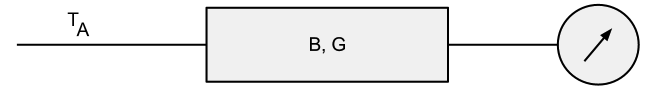
\includegraphics[width=\textwidth]{Images/simple_rad.png}
\isucaption{The ideal radiometer block diagram}
\label{simplerad}
\end{figure}
}

Figure~\ref{simplerad} shows us an ideal radiometer.  That is a radiometer that has an input from the antenna, T$_{A}$, a known bandwidth denoted as B and a known gain denoted as G.  At the end of the block is the detector, which measures the power from the radiometer.

Only a certain selection of the radio spectrum is observed by the radiometer.  This is referred to as the bandwidth of the radiometer and is denoted as B or as $\beta$.  This bandwidth is then centered around a center frequency.  In our case, we center around 1.4125 GHz.  There is a reason why 1.4125 GHz is selected.  The range from 1.4000 to 1.4260 GHz is protected internationally.  This reduces interference from outside sources such as transmitters that can interfere with the operation of the radiometer.  

The power coming from the antenna is amplified so it is easier to determine changes in the brightness temperature.  The overall gain of the radiometer system is referred to as G in this case.  Finally, we need to apply Boltzmann's constant, referred to as \textit{k}.  With these values, we can now compute the power the radiometer will see for an ideal radiometer.  This can be shown in equation~\ref{eq:power_rad_eq}

\begin{equation} \label{eq:power_rad_eq}
P=k*\beta*G*(T_{A})
\end{equation}

However, since we do not have an ideal radiometer, we have another key component that needs to be addressed.  This is the noise that is added to the system by the radiometer itself, primarily from the amplifiers used to increase the signal.  Most of the additional noise is from the Low Noise Amplifiers (LNA) that are used to increase the signal while attempting to keep the noise added to a minimum.  However, noise is also added from virtually every component in the RF front end.  However, by far the largest contribution usually comes from the LNA, which is why the selection of the LNAs is a critical decision.  Figure~\ref{noiserad} shows the additional noise that is injected into the system.

{\begin{figure}[h!tb] 
\centering
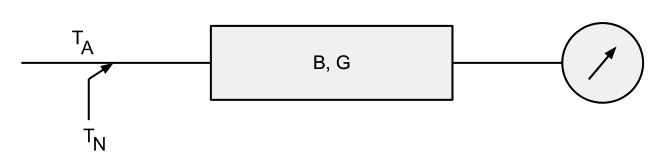
\includegraphics[width=\textwidth]{Images/radiometer_noise_added.png}
\isucaption{A more realistic radiometer model}
\label{noiserad}
\end{figure}
}

As it can be seen, this additional noise is added to the noise coming from the antenna source.  Therefore T$_{N}$ is added to T$_{A}$ and our final equation for the power measured is shown in equation~\ref{eq:final_power}.  

\begin{equation} \label{eq:final_power}
P=k*\beta*G*(T_{A}+T_{N})
\end{equation}

The issue with all radiometers is that it must detect small signal changes in a noisy environment.  To understand this, let us look at the example of T$_{A}$ has a value of 200 K and T$_{N}$ has a value of 800 K.  Since T$_{N}$ is added to our antenna signal, we have a total noise temperature of 1,000 K.  This means that if we want to detect a change as small as 1 K, we must be able to measure the difference between 1,000 K and 1,001 K. [\cite{skou}]

The ability of a radiometer to detect these small changes is the radiometer's sensitivity, or the standard deviation of the output signal from the radiometer.  This sensitivity is also referred to as the Noise Equivalent $\Delta$ Temperature or NE$\Delta$T and is shown in equation \ref{NEAT_EQ}. 

\begin{equation} \label{NEAT_EQ}
NE\Delta T=\frac{T_{A}+T_{N}}{\sqrt{\beta * \tau}}
\end{equation}

The sensitivity of the radiometer is based on both the bandwidth, $\beta$, of the incoming signal and the integration time, $\tau$.  As it can be seen in the equation, we would want to have as much bandwidth as possible.  In a traditional radiometer, this bandwidth is often fixed and is dependent on the band-pass filters used in the radiometer.  We can however control $\tau$ and a longer integration time will help improve the sensitivity of the radiometer.[\cite{ulaby}]

This covers a very simplified radiometer, however most radiometers are more complicated than the one shown in Figure~\ref{noiserad}.

{\begin{figure}[h!tb] 
\centering
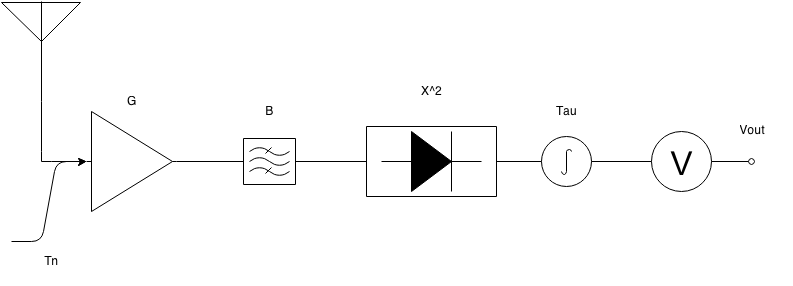
\includegraphics[width=\textwidth]{Images/Radiometer.png}
\isucaption{A total power radiometer}
\label{trad_radiometer}
\end{figure}
}

A more typical radiometer can be shown in Figure \ref{trad_radiometer}.  Here we have expanded the blocks used and have separated the bandwidth and gain blocks.  In addition, we have detection, shown as X$^2$, and integration.  These last two blocks make up the detection and results in the power we can measure, which is a voltage represented as V$_{out}$.  This results in equation~\ref{eq:vout_1}.  In most cases the detection is performed by a square-law detector[\cite{Leinweber}].

\begin{equation} \label{eq:vout_1}
V_{OUT}=c*(T_A+T_N)*G
\end{equation}

Here V$_{OUT}$ is shown by the addition of both the noise from the system T$_N$ and the noise from the antenna, T$_A$ and multiplied by the gain in the system, G.

The voltage output from this radiometer is then either measured or may also be sampled by an analog to digital converter.  In both cases the output has no real meaning until it is calibrated.

\section{Traditional Radiometer Theory of Operation}
The RF front end used in this thesis was originally built by the University of Michigan, however this later proved to be unreliable and was changed out to one that was designed and built by the author.  This RF front end was designed to be low cost while still maintaining excellent noise performance.  To do this, the RF Front end was designed to be very minimal, only using some basic filtering and the amplification needed so the power can be detected by the SDR.  The LNAs play an important role as explained in the previous section to amplify the noise we are looking at while minimizing the amount of noise they contribute to the overall system.  While band-pass filters would not need to be there, since we can filter with digital filters, they did ensure that the signal was in our area of interest.

\subsection{RF Front End Design}

The RF front end plays a critical role in a radiometer as the primary function is to amplify the signal so that it is easier to detect the changes in power or noise temperature.  Of course the amplification comes with a cost that the the LNA itself will contribute to the noise and this contribution is unwanted.  Therefore we want to minimize the contribution and maximize the amplification of the noise we are looking at.  The Noise Figure (NF) is a metric we use to show how well a LNA amplifies a signal while keeping it's contribution to the noise to a minimum.  Well engineered LNAs are now capable of producing very low noise figure numbers and are relatively inexpensive.  


A typical design is a 3 stage system that uses 2 bandpass filters to help maintain the signal to the band of interest.  A traditional radiometer requires the use of bandpass filters since most LNAs have a fairly large operating bandwidth.  The filters ensure that the radiometer is operating in the band of interest, in our case the L-band from 1400 to 1426 MHz.  

The software defined radio radiometer however does not require bandpass filters added.  There are two reasons for this.  One, the sampling rate set on the software defined radio sets a bandwidth and thus will limit the frequencies we are listening to.  Second, if needed additional filters can be created in software.  There is a cost to these filters in that additional processing power is needed, but otherwise they can be added with no additional cost to the system. 

\subsection{Existing ISU RF Front End}

The existing ISU radiometer RF Front end uses a series of cascading low noise amplifiers (LNAs) that increase the power from the antenna while contributing a minimum amount of noise to the system [\cite{Erbas}].  In addition, the current ISU RF front end uses bandpass filters to narrow the bandwidth to the desired 1400 to 1425 MHz that we wish to monitor.  While these are not needed with the addition of the software defined radio, since we can filter in software, they do not contribute much in terms of the noise temperature, and as passive components do not impact the performance of the radiometer as much as the LNAs do.

{\begin{figure}[h!tb] 
\centering
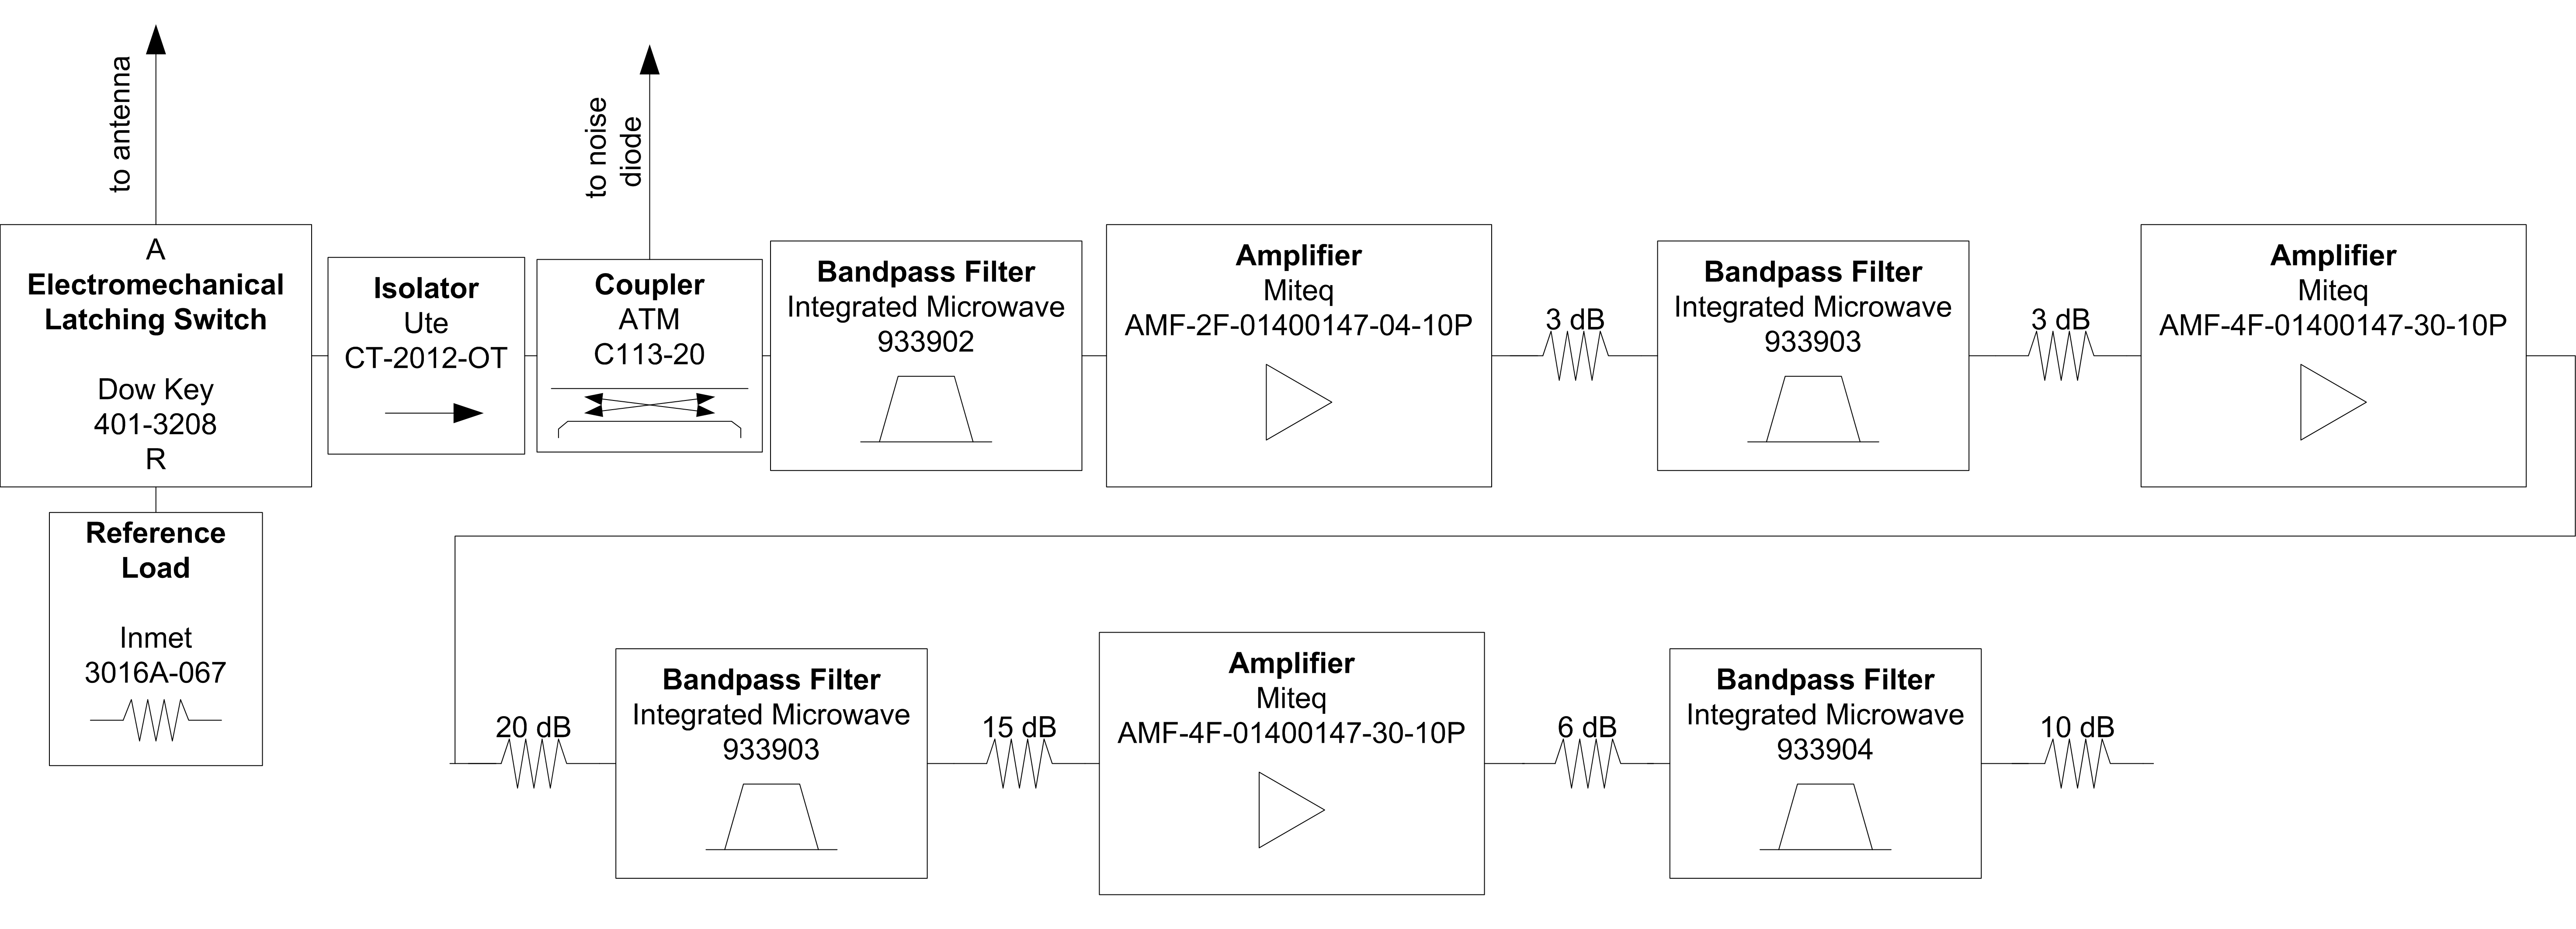
\includegraphics[width=17cm]{Images/ISU_rf_block.png}
\isucaption{A block diagram provided by the University of Michigan that shows the components used in the ISU RF front end.}
\label{ISU_rf_block}
\end{figure}
}

As it can be seen in Figure \ref{ISU_rf_block} the current ISU rf front end uses a series of amplifiers, filters and attenuators to amplify and filter the incoming signals.  The attenuators are used to ensure that we do not overload the front end of the LNA proceeding it in the chain.  This RF chain provides us a spectrum from 1400 MHz to 1425 MHz and gives us a total gain of approximately 81 dBm.  This raises the noise floor to approximately -30 dBm which makes it very easy to detect with both a square-law detector and the software defined radio.  The performance of the ISU front end was confirmed by using a spectrum analyzer to look at the output signal and power output.  The spectrum analyzer output can be seen in Figure 

{\begin{figure}[h!tb] 
\centering
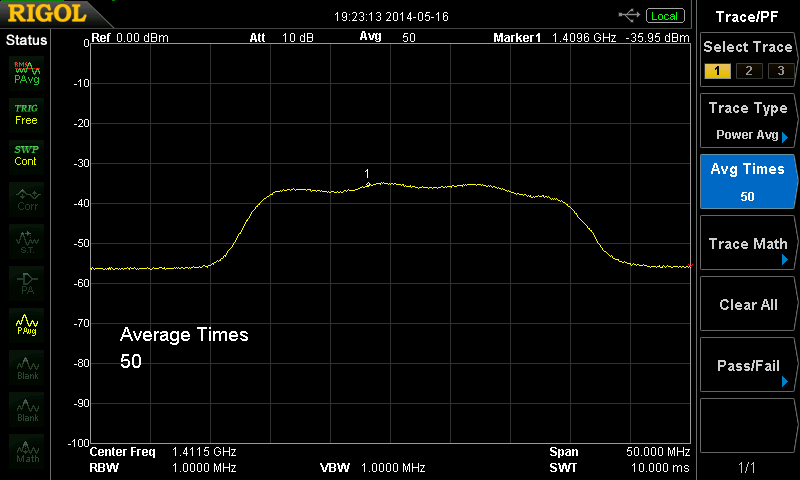
\includegraphics[width=17cm]{Images/radlidoff.png}
\isucaption{A screenshot taken from a spectrum analyzer showing the filters and amplification done by the ISU Radio RF front end.}
\label{ISU_rf_spectrum}
\end{figure}
}

The ISU Radiometer front end was dismantled and was used for the experiments used in this thesis.  The LNAs and bandpass filters were kept intact to be used for experimentation.  While the bandpass filters were not needed for the software defined radio, since we were comparing our data to a square-law detector, they were still required for that device so that both the SDR and the Square-law detector could be looking at approximately the same signal.

\subsubsection{A note about the ISU RF Front end}

During the work on this thesis a few issues came up with the ISU RF front end that was used.  When work began on this thesis, it was assumed that the problems that were found with this hardware was limited to the digital portion of the radiometer.  This meant that the RF front end was performing as expected.  At first, early tests on the ISU RF front end seemed to confirm this as the output seen on a spectrum analyzer appeared to be normal.  However, further testing started to show unusual behavior.  Later, it was discovered that the ISU RF front end was prone to malfunctioning under certain conditions.  These conditions seemed to occur when the RF front end was moving on it's platform and even the lid to the box containing the RF front end would affect it.  

A test was done to show this effect with the lid, and further information about the rotation affect is discussed in Appendix 2 in regards to the E E 518 laboratory experiment. For the lid experiment, a spectrum analyzer was hooked up to the ISU RF front end.  With the lid off, you can see what appears to be a normal signal that we would expect from the radiometer in Figure \ref{ISU_rf_spectrum}.  However, in Figure we placed the lid on the radiometer and the results are quite different.  Changes to the signal were observed in real time as the lid was placed on the radiometer and it was clear that this was also causing the radiometer to produce undesirable results.  

{\begin{figure}[h!tb] 
\centering
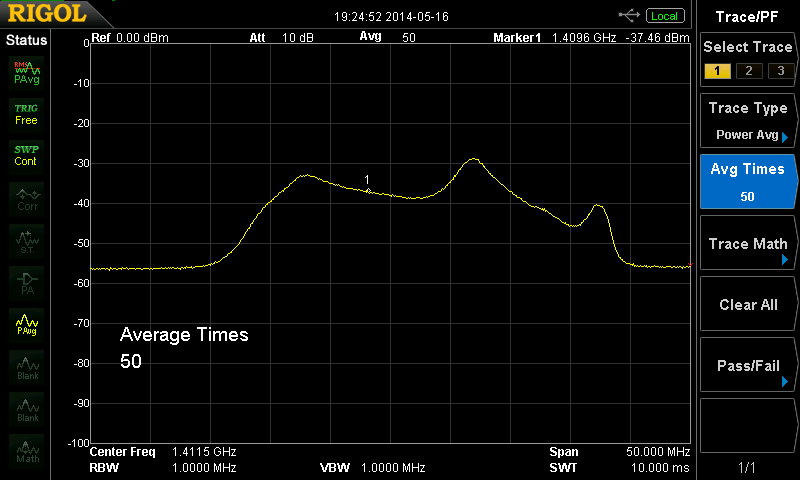
\includegraphics[width=17cm]{Images/lidpart.png}
\isucaption{A screenshot taken from a spectrum analyzer showing the affect of the radiometers lid as it was placed on the radiometer.}
\label{lid_on}
\end{figure}
}

It was clear that there is something happening with the ISU RF front end.  This also points out another use for the addition of the software defined radio.  The old ISU radiometer system under-sampled the signal and so frequency information was lost.  Without hooking up something like a spectrum analyzer there would be no way for any to know what was happening with the ISU radiometer.  However, with the SDR we now have power and spectrum information.  In fact, it was during the E E 518 laboratory that we noticed a problem with the ISU radiometer and we discovered this by looking at the data that was captured by the SDR.  It was due to these issues that came up that the RF front end was rebuilt. 

Work was done to re-stabilize and make the ISU radiometer front usable for the experiments used in this thesis.  First, all non-essential equipment was deactivated and powered down.  This included the on board microcontroler, the A/D converters and the FPGA unit that was originally used in this radiometer.  The thermal electric coolers were also deactivated as well.  Since the LNAs were in a temperature controlled room, they were not needed for these experiments.  

Next, the LNAs were powered from a lab bench power supply instead of the power supplies that were used in the radiometer.  It is theorized that the power supplies feeding the radiometer may have been damaged due to water that had entered the case and were no longer stable in the power they provided.  To eliminate any issues, they were removed and a new and known to be working lab power supply was used to power both the LNAs and the square-law detector circuitry.   

\section{Software Defined Radio Theory of Operation}

A software defined radio (SDR) attempts to mimic radio functions in software instead of relying on dedicated hardware.  As stated in the previous section, a radiometer is a radio that can detect changes in power.  Therefore the SDR needs to be able to measure power coming from the source that we are looking at.  

The SDR is able to do all of this but in a slightly different way than a traditional radiometer.  A traditional radiometer will use a device called a square-law detector to measure the incoming RF signal.  This device is simply a diode where the input voltage is squared and the output from the diode is proportional to the AC input voltage.  Therefore a 3 dB increase in the RF power will result in a two times increase in the voltage.  This power measurement will be fluctuating rapidly, therefore we will then run the output from the square-law detector to an integrator and integrate over a set time period.  As shown in equation \ref{NEAT_EQ}, this integration time also affects the NE$\Delta$T or sensitivity of the radiometer as well.

For the SDR, the incoming signal is sampled and converted to I/Q values.  The I/Q values represent the amplitude and phase information of the signal.  In GNURadio we are then able to square these values within software.  This block in GNURadio mathematically performs what is shown in equation \ref{sdr_x2}.

\begin{equation}\label{sdr_x2}
I^2+Q^2 = P_{out}
\end{equation}

Like the analog square-law detector, this signal will fluctuate rapidly and to improve the sensitivity of the radiometer we wish to integrate this signal.  A RC filter is analogous to an integrator where the R and C values determine our time constant and our integration time for the filter.  A SDR however operates in the digital domain at discrete intervals.  One type of filter that can be used in the Infinite Impulse Response (IIR) filter. 

To begin with, we look at what an analog RC filter looks like. 

{\begin{figure}[h!tb] 
\centering
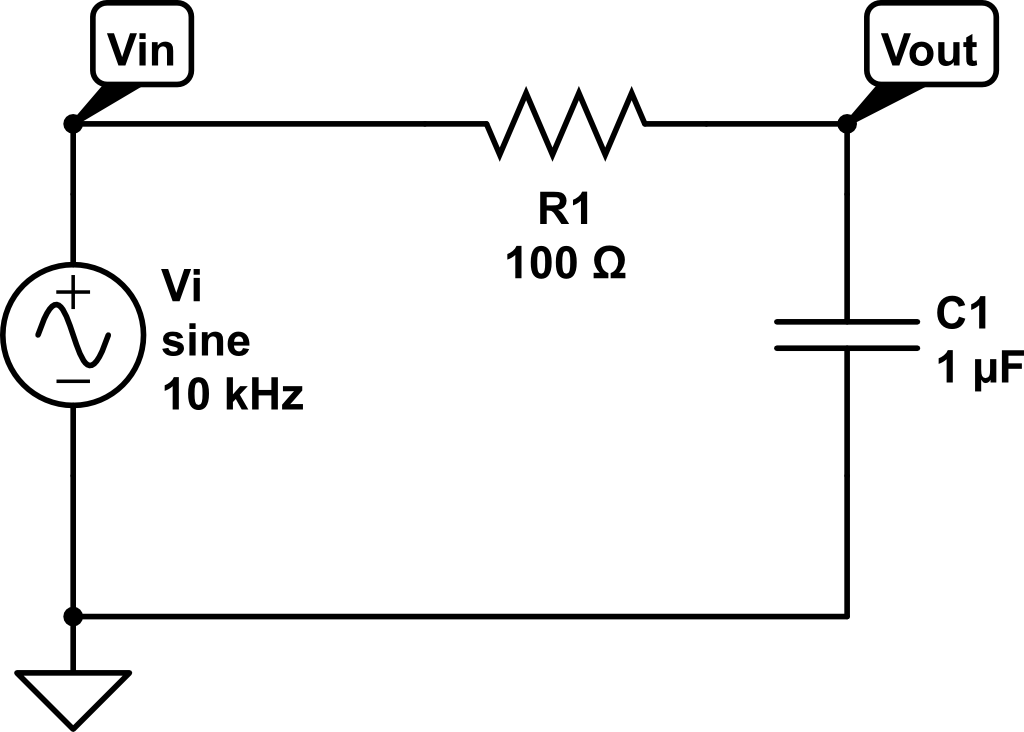
\includegraphics[width=10cm]{Images/rc-circuit.png}
\isucaption{A simple RC circuit}
\label{rc_circuit}
\end{figure}
}

This circuit can be represented by equation \ref{eq:rc_circuit_eq}.

\begin{equation}\label{eq:rc_circuit_eq}
\frac{V_{in}-V_{out}}{R}=C\frac{dV_{out}}{dt}
\end{equation}

A Finite Impulse Response (FIR) filter is a digital filter that can take an impulse signal and decays to zero after a finite number of iterations.  This type of digital filter can be represented by equation \ref{FIR_Eq} which mathematically expresses the FIR Filter.

\begin{equation}\label{FIR_Eq}
y_n=\displaystyle\sum\limits_{i=o}^{P-1} c_ix_{n-i}
\end{equation}

This simply says that the nth output is a weighted average of the most recent P inputs.  

An Infinite Impulse Response (IIR) filter is the same as the FIR filter, except that we add an additional summation term which feeds back the previous output.

\begin{equation}\label{IIR_eq}
y_n=\displaystyle\sum\limits_{i=o}^{P-1} c_ix_{n-i}+\displaystyle\sum\limits_{j=1}^{Q} d_jy_{n-j}
\end{equation}

Equation \ref{IIR_eq} shows that a FIR filter is really a IIR filter, except that $Q=0$.  

To get a better understanding on how our digital IIR filter relates to our RC filter analog, we can look at the Fourier Transform and the relationship of the input to the output in the frequency domain.

\begin{equation}\label{Fourier_IIR}
H(f)=\frac{\displaystyle\sum\limits_{j=o}^{P-1} c_je^{-2\pi ijfT}}{1-\displaystyle\sum\limits_{k=1}^{Q} d_ke^{-2\pi ikfT}}
\end{equation}

In equation \ref{Fourier_IIR}, $f$ is our frequency in Hz and $T$ is the time between samples in seconds and is related to our sampling frequency.

We now want show the link between our analog RC circuit and the IIR filter.  Looking at equation \ref{eq:rc_circuit_eq}, which represents the differential equation relating the input voltage $V_{in}$ to the output voltage $V_{out}$, we can substitute for input and output of our IIR filter.  Since we are now in the time domain, we need to define what $T$ is and we can do that using equation \ref{sampling_rate_eq}.

\begin{equation}\label{sampling_rate_eq}
T=time between samples=\frac{1}{sampling rate}
\end{equation}

We can now relate our input voltage to the input to our IIR filter and the output voltage to the output of our IIR filter.

\begin{equation}\label{input_IIR}
x_n=v_{in}(nT)
\end{equation}

\begin{equation}\label{output_IIR}
y_n=v_{out}(nT)
\end{equation}

We can now rewrite our difference equation with $x_n$ and $y_n$.

\begin{equation}\label{diff_xn_yn}
\frac{x_n-y_n}{R}=C\frac{y_n-y_{n-1}}{T}
\end{equation}

Now, we can solve for $y_n$ which results in our final equation for showing how a IIR filter is related to an RC filter.

\begin{equation}\label{final_IIR_RC}
y_n=\frac{T}{T+RC}x_n+\frac{RC}{T+RC}y_{n-1}
\end{equation}

It can be seen that an IIR filter can have the same frequency response as we would expect from an analog RC filter.  As our sampling rate approaches infinity, the approximation gets closer to the original response from the analog RC circuit.  

For the cutoff frequency of a RC circuit, we know that it has the relationship shown in equation \ref{RC_relationship}.

\begin{equation}\label{RC_relationship}
f_c=\frac{\sqrt{3}}{2\pi RC}\rightarrow RC=\frac{\sqrt{3}}{2\pi f_c}
\end{equation}

The $RC$ term gives us our time constant of the circuit and can be used to calculate out our coefficients.  We are not concerned about the actual values of R and C with our IIR filter, instead we just need the product of R and C.  

For GNURadio most of the work is done for us.  We can simply enter in our desired cutoff frequency and GNURadio will calculate our IIR filter coefficients.  However, this shows that an IIR filter works very much like an analog RC low pass filter.

Like a traditional radiometer, the SDR will use an antenna to look at the target of interest.  SDRs still use a RF stage that takes the power from the source and amplifies it.  The difference though begins after that.  A SDR will then sample and generate I and Q values that represents the amplitude and phase of the signal.  From there, this data is sent to a computer to be processed.  We can then use this information to calculate the power that is being seen.  In addition, we can manipulate the signal in other ways such as applying a filter to filter out an unwanted source.

Now that we have the un-calibrated power and we have applied a low-pass filter to smooth out the information, we have replicated the key components that you would find in a traditional radiometer.  All of this has now taken place in the digital domain.  The information can now be stored, displayed or both for further analysis.  
\subsection{General Specifications}

The N200 is a SDR developed and built by Ettus Research.  It is one of the newer models in the companies USRP line of SDRs.  It offers several key features that were desirable for a radiometer type of application while still being an economical option.  It also offered a highly flexible architecture which will allow this radio to be up-gradable in the foreseeable future.  

{\begin{figure}[h!tb] 
\centering
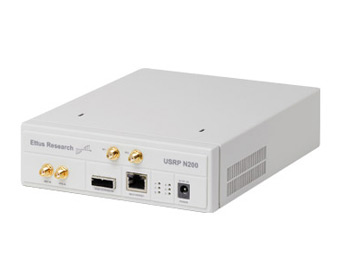
\includegraphics{Images/n200}
\isucaption{The USRP N200 from Ettus Research}
\label{N200}
\end{figure}
}

The N200 has the following features that made it well suited for our specific application.

\begin{itemize}
\item Dual 14-bit ADC
\item Dual 16-bit DAC
\item 50 MS/s Gigabit Ethernet streaming
\item Modular daughter-board system for RF front end
\end{itemize}

These specifications had a large impact on the selection of the N200 for this application.  Specifically the 14-bit ADC, the 50 MS/s and the modular daughter-board system were the largest factors in the decision to use the N200 SDR.  Further explanation on these specifications are explained in the following sections.

\subsubsection{14-bit ADC}
The analog to digital converters (ADC) allow us to take the analog I and Q values from the daughter boards and digitize this information.  Once digitized, we can now work with the signal both on the on-board FPGA board or stream it to the computer so that our software can manipulate the signal.  In radiometry, we are primarily looking at the overall power of the signal and this does not require us to accurately recreate the signal.  However, it will be discussed in this paper in further detail that there are times where being able to recreate the signal for additional analysis can be quite beneficial.  For that reason, the resolution of the ADC becomes more important.

\subsubsection{50 MS/s Bandwidth}
For this application, the N200 is required to receive a signal at 1.4 GHz and is at least 20 MHz wide.  Bandwidth plays an important role in remote sensing and to the amount of power that we receive.  It also plays a key role in the sensitivity of the radiometer.  This was discussed in the theory of a traditional radiometer and equation \ref{eq:final_power} shows us the relationship that our bandwidth plays in the overall power received.    

Equally important however is the the sensitivity or how small of a change the radiometer can detect.  This sensitivity or NEAT function is shown in equation \ref{NEAT_EQ}.  Again, the amount of bandwidth the radiometer receives plays a large part in the performance of the radiometer.  

Another factor however is the amount of bandwidth the existing RF front end of the ISU radiometer is able to provide to us.  The current filters on the ISU Radiometer keep the bandwidth of the signal to 20 MHz.  This meant that at the very minimum a 20 MS/s bandwidth from the SDR is required.  

The N200 is capable of working with up to 100 MS/s signal and can stream up to 50 MS/s through the Gigabit Ethernet connection.  The N200 also has the ability to have up to 2 daughter boards installed.  If we assume each will have up to a 20 MHz signal, this means up to 40 MS/s of data will be required.  This means that the N200 meets are minimum requirements for working with needed bandwidth of the radiometer.  In addition, the FPGA on the N200 is capable of working with up to 100 MS/s, so there is room handling additional bandwidth by using the on board FPGA to process the signal.

\section{A Software Defined Radio Radiometer Theory of Operation}
A software defined radio radiometer implements the key features of a radiometer in software instead of relaying on hardware.  While some hardware is still needed, primarily with the RF front end that amplifies the signal while maintaining a low noise factor, we want the software to do as much of the work as possible.  

\subsection{Hardware}

Hardware with a software defined radio still plays a critical role.  A traditional software defined radio will focus on digitizing the signal as soon as possible and the hardware used will be focused on performing that critical digitizing process.  For a software defined radio radiometer, we still want to digitize as soon as possible, but we also need to consider our noise factor.  Most software defined radios are designed for communication purposes such as implementing 802.11b or other wireless protocols.  In these cases a higher noise factor is not as detrimental to the overall system as it would be with a radiometer.  This is mainly due to the fact that we have a known signal that is magnitudes greater than the noise floor.  In a radiometer however, we do not have this large separation between the information we need and the noise of the system.  And so our noise factor is a more critical component.  

To counter this, we use Low Noise Amplifiers to amplify the signal but it can also help lower our noise factor.  The first LNA in the chain contributes significantly to our noise factor, so by selecting a LNA that has a very low noise factor, it reduces the noise factor for the system.  This can be shown by looking at the equation that calculates our noise factor.

\begin{equation}\label{noise_factor}
F=F_1+\frac{F_2-1}{G_1}+\frac{F_3-1}{G_1 G_2}+\frac{F_4-1}{G_1 G_2 G_3}+\cdots +\frac{F_n-1}{G_1 G_2 G_3 \cdots G_{n-1}}
\end{equation}

This however is the only major change we need to do for doing radiometer work with an off the shelf radiometer.  The rest will be done within software which is the principal reason for using a software defined radio.  

The rest of the hardware that is needed is the hardware to allow us to digitize the signal as soon as possible.  The Ettus Research N200 SDR uses daughter boards which allow for easy replacement of the RF front end to the software defined radio.  Ettus Research makes a number of daughter boards that range from a a wide range of frequencies and is available with transmitters, receivers and transceivers.  Because these boards are modular and do not touch the analog to digital converters or the on-board FPGA, very little change is required in the software.  The daughter boards however do have the required RF hardware for the signal to be processed.  In this application it was required that the signal was detected at 1.4 GHz with a bandwidth of 20 MHz.  The DBSRX2 receiver met this requirement and was selected to be used with the N200.  In this radiometer application transmission is not needed and is in fact illegal in the 1.4 GHz band, which is reserved for radiometer applications.

\subsubsection{The DBSRX2 Receiver}
The DBSRX2 receiver board is capable of receiving signals between 800 MHz and 2.3 GHz.  The board is able to plug into one of expansion slots available on the N200 that we are using.  This board then down-coverts the signal into analog I and Q values that are then fed into the N200 analog to digital converter.

{\begin{figure}[h!tb] 
\centering
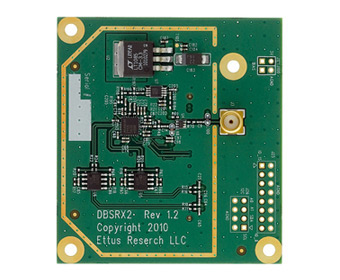
\includegraphics{Images/dbsrx2}
\isucaption{The DBSRX2 daughter board from Ettus Research}
\label{dbsrx2}
\end{figure}
}

The DBSRX2 has several key components on it that is used to take the analog RF signal and prepare it for digitization by the analog to digital converter.  First the signal is amplified through a Programmable Gain Amplifier (PGA).  This PGA is accessible from the software and can be configured by the software.  Next the signal goes into a direct-conversion integrated circuit that directly converts the RF signal to analog I and Q values.  The integrated circuit, a Maxim MAX2112 device, also includes a Low Noise Amplifier (LNA), mixer and Low Pass Filter (LPF).  This essentially amplifies the signal, mixes into baseband and then applies a low pass filter.  

These analog I and Q values are then passed to the N200 to be sampled by the analog to digital converter.  The IQ values are differential signals to minimize noise possible interference.

\subsection{Software}
Software of course plays a critical role in both a software defined radio but also in our software defined radio radiometer.  There are really two pieces of software that are in play with the software defined radio we are using.  The first is the firmware that used in the FPGA of the N200.  However, this firmware currently does not implement the actual radiometer functions but instead provides us a link to both the I/Q data and also the control of the of the SDR itself.  

The second is the software that is running on the host computer.  It is this software that provides the calculations on the I/Q data to give us the information we need and also creates a GUI for the user to interface with the radio.  For this software, we will be using GNURadio, an open source software program that is used in many software defined radios including the N200 SDR that we have.

\subsubsection{GNURadio}

GNURadio fills in the software side of the software defined radio.  Although there is firmware that runs on the FPGA in the N200, this firmware is designed to communicate with a host PC.  It is this software that does most of the work in terms of the calculations that are done with the signal.  The FPGA simply sends the raw IQ data to the host PC, which then performs the necessary math functions.  Again, the reason why software defined radios are desirable is the ability to change the behavior of the radio very quickly.  In our case we can change functionality by simply loading a new software program in the host PC.  

This functionality is ideal for communication type of radios where different modulation schemes and encoding and decoding methods can easily be changed out.  However, in a radiometer we are not interested in this aspect of the SDR.  However, one functionality is available that can be very valuable for a radiometer, and that is with filtering.  Although we often use frequencies that should be free from interference, this is not always the case.  Interference can and often does still occur, even in these protected frequencies.  With the SDR, we are able to quickly adapt to changing conditions by moving the frequency, changing our bandwidth and even filter out an offending signal.  

GNURadio was selected as it is an open source software platform.  GNURadio is licensed under the GPL license and has a strong community that continually updates the software.  It is also well supported by third parties such as Ettus Research Group, National Instruments and other SDR developers.  In addition GNURadio has a strong set of tools that can be used to develop programs that run under GNURadio.  Tools such as the GNURadio Companion (GRC) allows for an easy to use GUI to develop code for GNURadio.  GNURadio is also written in Python, which allows for easy modification and access to additional tools that can be used with GNURadio.  

{\begin{figure}[h!tb] 
\centering
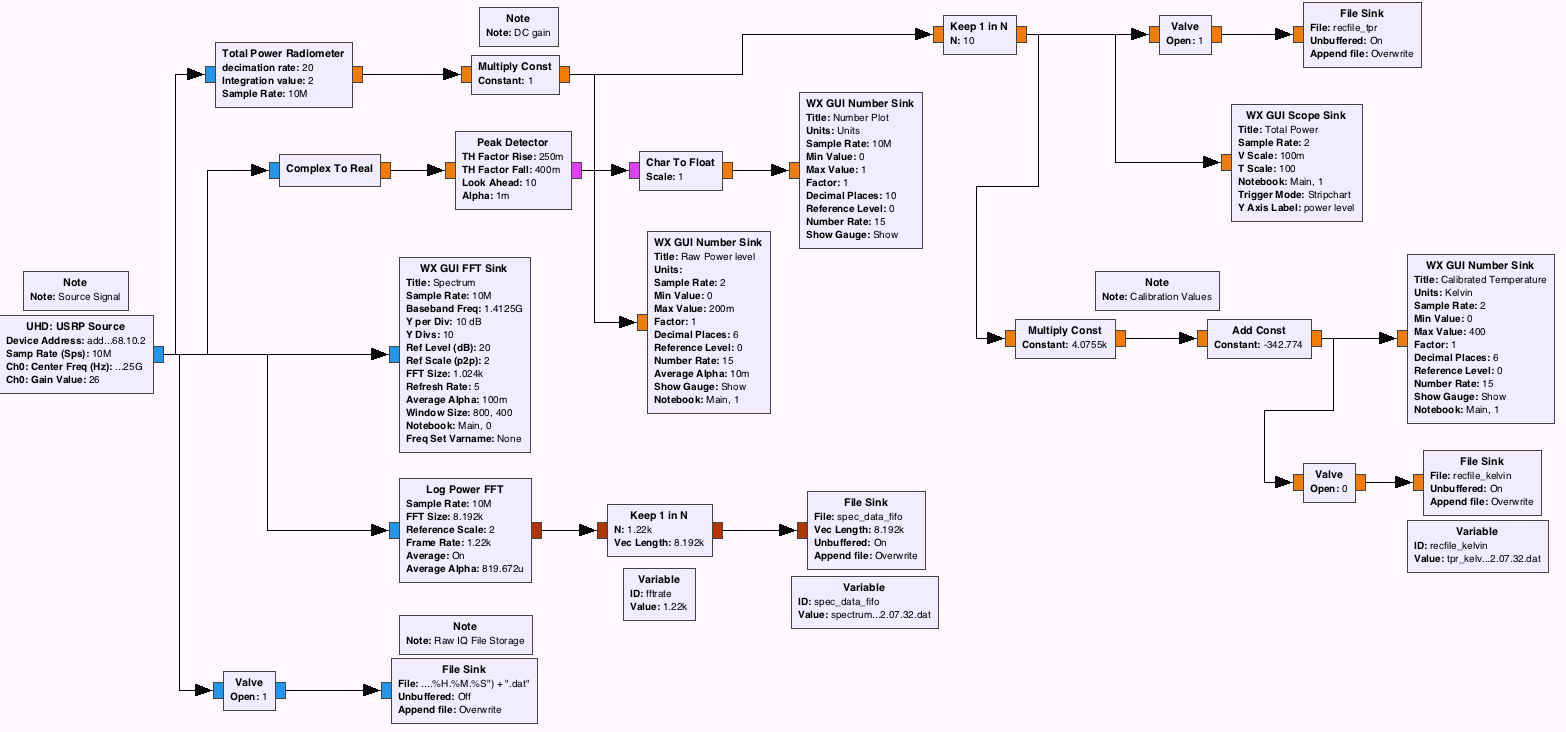
\includegraphics[width=17cm]{Images/N200_radiometer_grc.png}
\isucaption{Screenshot of the GNURadio Companion editor and the N200 Radiometer block diagram used in many of the experiments}
\label{N200_GRC}
\end{figure}
}

GNUradio Companion works by having many of the common functions as blocks that can picked and placed on the screen.  Once placed, the blocks can be wired up, very much like LabView, and the flow of data can be controlled in this fashion.  While GNURadio Companion provides most of the essential blocks used in most applications, additional blocks can by added if needed.  This is due to the fact that GNURadio is built using Python and the blocks in GNUradio Companion are simply blocks of Python code.  To "compile" a GNURadio Companion sheet, you simply run the sheet, which then generates the Python code that is then executed.  GNURadio actually uses a combination of Python and C++, where Python handles most of the interface and the C++ is usually most of the drivers and low level interface to the hardware.  This allows for a easy to use system but still meets some of the demanding performances needed for handling large amounts of data.  

GNURadio Companion also includes blocks that allow it to create a GUI type of interface.  The typical method it uses for this is using wxGUI although GNURadio Companion does also include blocks that can use QT for generating widgets as well.  However, the wxGUI tends to work better and has better support in GNURadio than QT.  

Through these blocks can not only manipulate the data we need to perform a total power radiometer in software but to also create a user interface that allows us to control the radiometer as well.  We are also able to display the information in real time so the user can see changes in power and even monitor spectral information during the operation of the radiometer. 

\section{Comparison of a Software Defined Radio Radiometer vs Traditional Radiometer}

As outlined above, a software defined radio implements a traditional radiometer but in the digital domain.  For power detection, we simply sum the squares of the I and Q values that have been sampled by the software defined radios analog to digital converters.  As with a traditional radiometer, we also want to filter this information to remove much of the jitters that comes from the rapid fluctuations in the power readings.  This is done using an IIR low pass filter, which mimics a traditional RC low pass filter.  Once completed, we now have the total power reading from the radiometer and we can now store, display or both this information.  

A traditional radiometer may also use an analog to digital converter in order to digitize the analog voltage from the square-law detector.  Because the sample rate of this voltage is very low, almost any analog to digital can be used for this.  At this point however, there is no frequency information, only the magnitude information is being retained and recorded.  

\section{Comparison of a Software Defined Radio Radiometer and other Digital Radiometers}

A digital radiometer is not a new concept.  Early radiometers would often digitize the analog voltage information from the square-law detector and then send that information to a computer for storage or analysis.  

A pre-cursor to a software defined radio, some radiometers would also digitize the incoming RF signal, but under-sample this information.  Since only power is the information desired this was acceptable.  However, these radiometers did often use the same components you might find in a software defined radio such as an A/D converter and FPGA.  These components however were used in different ways.

One reason why these devices were used differently from a SDR was due to cost.  Most radiometer operations happen at 1.4 GHz or above.  A/D converters at these higher frequencies become more expensive and harder to obtain.  In recent years however, these costs have come down.

The major difference between other digital radiometers and what is discussed in this thesis is that we retain both phase and magnitude information and instead mimics a traditional radiometer in software by summing an squaring the I and Q values and then running this information through a low-pass IIR filter.  By retaining this information, we can perform a more in-dept analysis of the signal coming into the radiometer which allows for greater agility in the system.